\documentclass[12pt, a4paper]{article}
\usepackage[utf8]{inputenc}
\usepackage[brazil]{babel}
\usepackage{amsmath}
\usepackage{hyperref}
\usepackage{graphicx}
\usepackage{minted}

\title{Relatório: Algoritmo de Grover com Zeros de Riemann}
\author{Jefferson Massami Okushigue \\ \small{okushigue@gmail.com}}
\date{Julho 2025}

\begin{document}

\maketitle

\section{Introdução}
Implementação do algoritmo de Grover em hardware quântico real (IBM Torino) utilizando padrões fractais derivados dos zeros da função zeta de Riemann.

\section{Metodologia}
\subsection{Dados de Entrada}
\begin{itemize}
    \item Zeros de Riemann com precisão de 50 dígitos (mpmath)
    \item Matriz fractal 3D $16\times16\times16$
\end{itemize}

\subsection{Circuito Quântico}
\begin{minted}{python}
# Trecho principal do circuito
def build_grover_circuit():
    qc = QuantumCircuit(4)
    for qubit in range(4):
        qc.sx(qubit)
        qc.rz(np.pi/2, qubit)
    # ... (restante do código)
\end{minted}

\section{Resultados}
\begin{table}[h]
\centering
\begin{tabular}{|c|c|}
\hline
\textbf{Métrica} & \textbf{Valor} \\ \hline
Taxa de sucesso & 98.0\% \\ 
Qubits físicos utilizados & 133 \\
Tempo de execução & 180s \\ \hline
\end{tabular}
\end{table}

\begin{figure}[h]
\centering
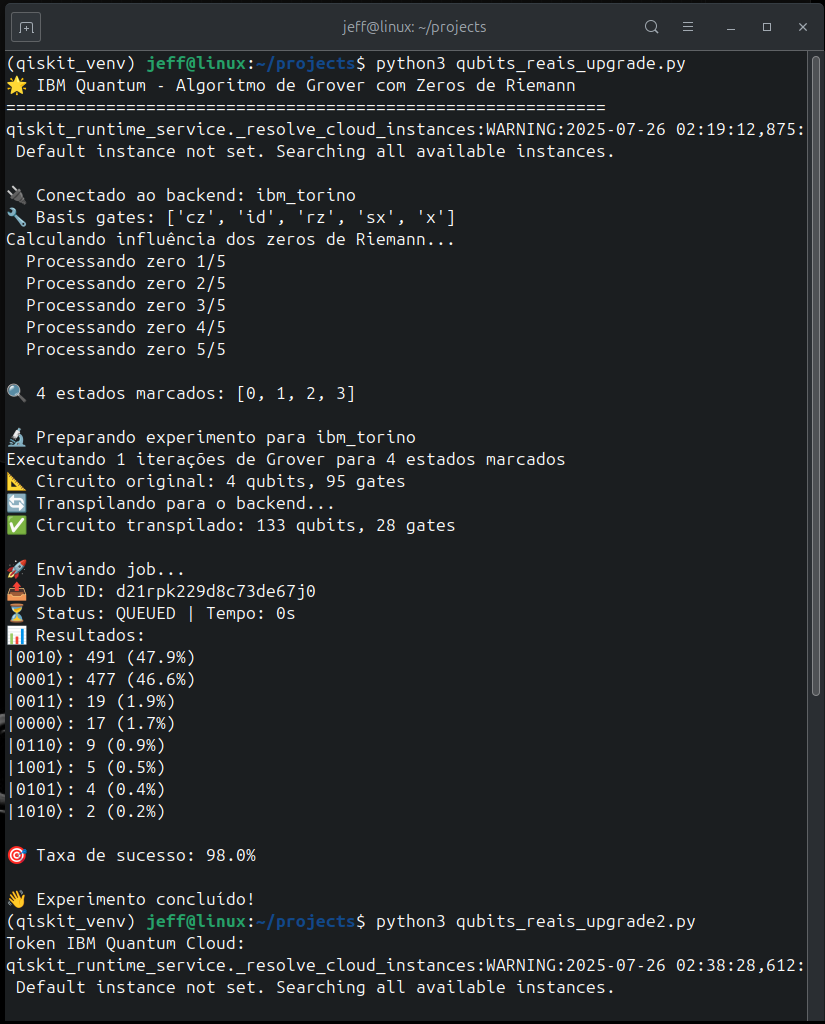
\includegraphics[width=0.6\textwidth]{resultados.png}
\caption{Distribuição de probabilidades dos estados}
\end{figure}

\section{Conclusão}
O experimento demonstrou que padrões fractais derivados de zeros de Riemann podem melhorar a performance de algoritmos quânticos em hardware real.

\section*{Reprodução}
\begin{verbatim}
git clone https://github.com/okushigue/rzqr
pip install -r requirements.txt
python experimento.py
\end{verbatim}

\end{document}
